% !TeX root = ../main.tex
% Add the above to each chapter to make compiling the PDF easier in some editors.

\chapter{Literature Review}\label{chapter:literaturereview}
This chapter provides a comprehensive review of the literature relevant to teleoperation interfaces for autonomous vehicles, focusing on environmental data visualization and perception modification. The review covers various topics, from the fundamentals of autonomous vehicle technology to specific teleoperation concepts and visualization approaches.
\section{Overview of Autonomous Vehicle Technology}

The Society of Automotive Engineers (SAE) International has defined six levels of
driving automation, as shown in figure 2.1 in their J3016 standard, which has become
the industry’s most widely accepted classification system. These levels range from 0
(no automation) to 5 (full automation), providing a clear framework for understanding
the capabilities of autonomous vehicles \cite{sae2021}

\begin{figure}[h]
    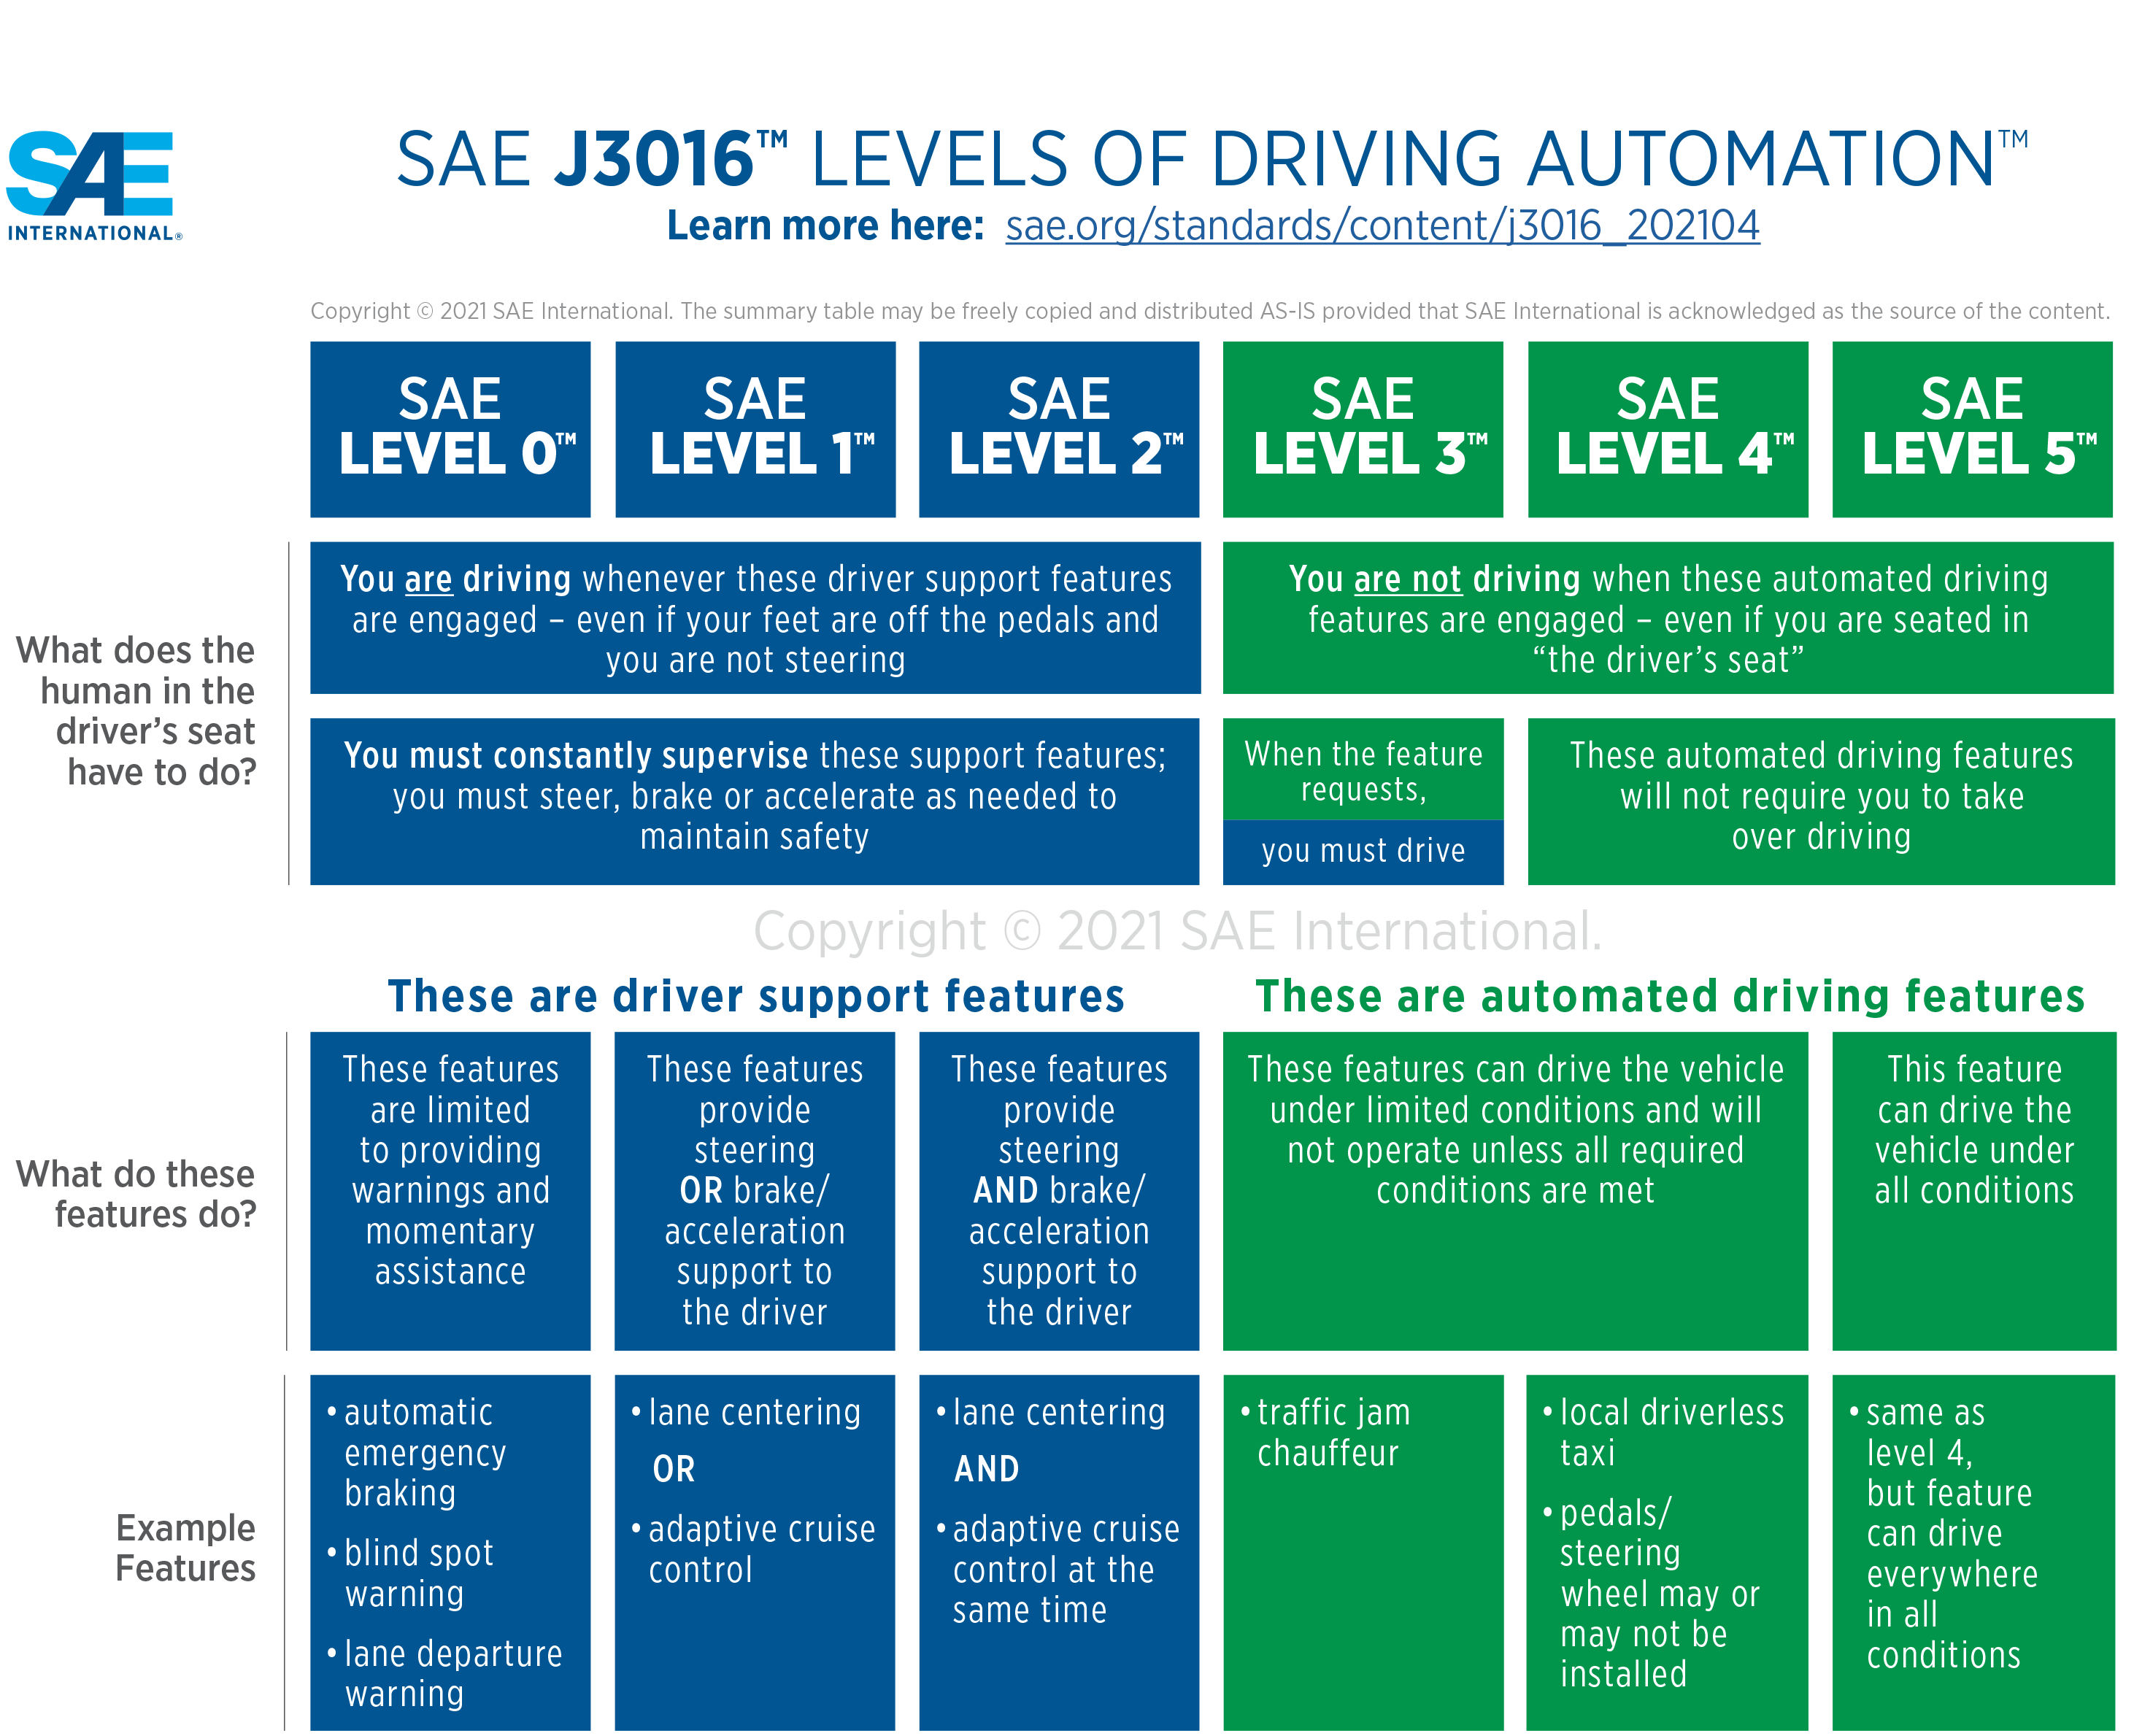
\includegraphics[scale=0.4]{figures/SAE.png}
    \centering
    \caption{SAE Levels of Automation \cite{sae2021}}
    \label{fig:SAE}
\end{figure}

As of 2024, most advanced consumer vehicles operate at Level 2, with some manufacturers pushing towards Level 3 capabilities. For example, BMW has recently become the first carmaker to receive approval for combining both Level 2 and Level 3 autonomous driving systems in a single vehicle. The new BMW 7 Series now offers the BMW Highway Assistant (Level 2) and the BMW Personal Pilot L3 (Level 3), marking a significant step in automated driving technology \cite{bmw2024}.

At the forefront of autonomous vehicle technology, companies like Waymo
are making significant strides towards Level 4 autonomy. Waymo has achieved
Level 4 autonomy in pilot areas, offering fully autonomous rides without safety
 drivers in cities like San Francisco, Phoenix, and Austin \cite{evmagazine2024}.

 Achieving higher SAE levels of autonomy requires a sophisticated autonomous driving stack,
 which is composed of several vital modules that work together to perceive the environment,
 make decisions, and control the vehicle. The stack typically follows a modular software
 architecture that is shown in Figure \ref{fig:AVStack} integrates hardware and software components to enable safe and
 efficient vehicle operation

\begin{figure}[h]
    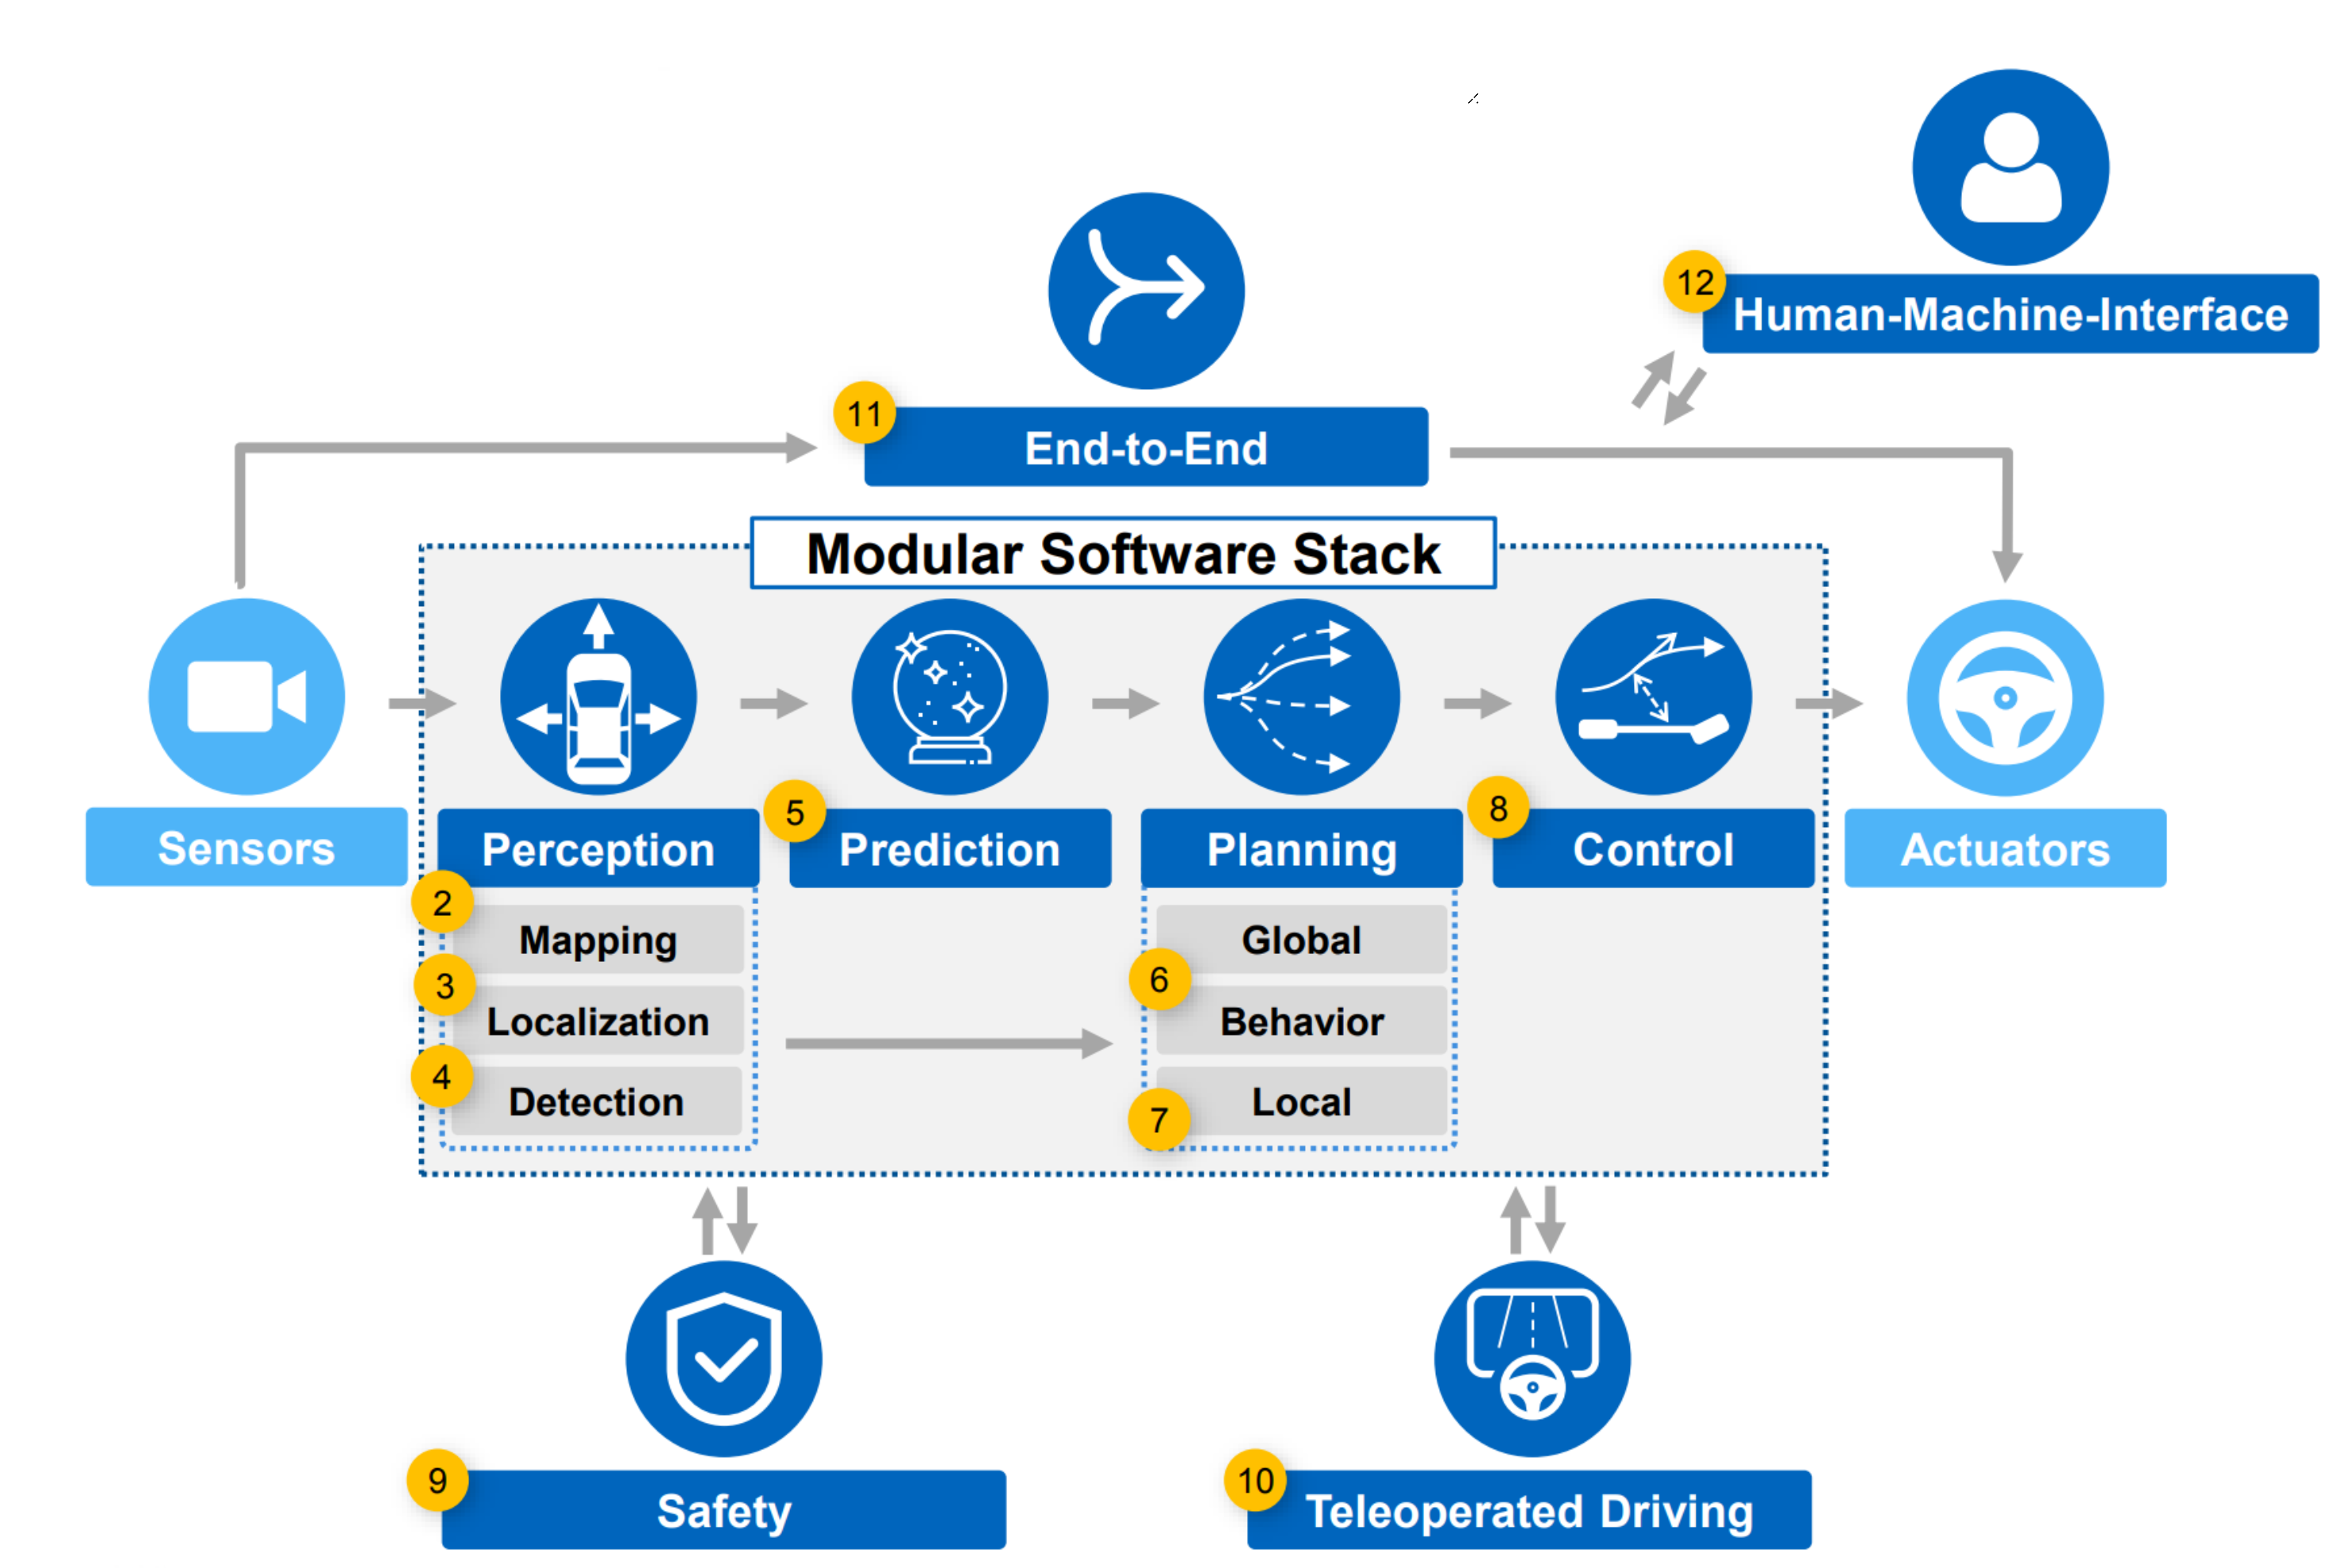
\includegraphics[scale=0.14]{figures/AVStack.png}
    \centering
    \caption{Autonomous Vehicle Technology Stack} %todo: add source from the lecture
    \label{fig:AVStack}
\end{figure}

While some research has explored end-to-end learning, where deep learning models directly map sensor inputs
to control outputs without modular decomposition \cite{codevilla2019limitations}, this approach alone is often
insufficient for achieving higher levels of autonomy. End-to-end systems can struggle with interpretability
and adaptability across diverse driving scenarios \cite{e2e}. It is an active research area and some
of the mentioned issues can be solved with Modular end-to-end learning \cite{nvidia2022diffstack} and also
it is expected to have a better performance on end-to-end methods with the improving hardware and datasets overtime \cite{e2e}.

For a system to reach higher SAE levels—particularly Level 4 or 5—all of
these modules must function reliably across various environments and conditions.
Each component plays a critical role in ensuring that the vehicle can navigate complex urban
environments safely and efficiently while responding to dynamic changes in real-time.
And we have teleoperation for the the cases where one or more module fails to deal the edge cases in the designed level of autonomy.
Teleoperation serves as a bridge between current autonomous driving capabilities and fully autonomous operation.
It allows vehicles to complete their missions even when their onboard systems encounter limitations.
For instance, if an autonomous vehicle encounters a situation outside its Operational Design Domain (ODD)\cite{iso34503},
such as unclear road markings or interactions with law enforcement, it can pull over safely and request human
intervention through teleoperation. This technology is essential for ensuring that autonomous vehicles
can operate reliably in real-world conditions and is expected to play a key role in the widespread adoption of autonomous vehicles.


\subsection{Types of Sensor Data in Autonomous Vehicles}
Autonomous vehicles rely on a range of sensors to perceive their environment and
gather the necessary data for safe and efficient navigation. These sensors provide
raw data that is processed by the vehicle's perception system to understand its
surroundings, detect obstacles, and make real-time decisions.
In the later sections we will refer these unprocessed data as "Raw data" or "Raw sensory data".
The key types of sensor data used in autonomous vehicles include:
\begin{itemize}
    \item \textbf{LiDAR (Light Detection and Ranging):}
    LiDAR sensors use laser pulses to measure distances between the vehicle and surrounding objects.
    By emitting laser beams and measuring the time it takes for them to reflect back, LiDAR creates
    a detailed 3D map of the environment. This technology is particularly useful for detecting objects'
    shapes, sizes, and positions with high accuracy, even in low-light conditions \cite{levinson2011towards}.
    LiDAR is widely used in autonomous vehicle systems due to its precision in mapping the surrounding area.

    \item \textbf{Radar}:
    Radar sensors use radio waves to detect objects and measure their speed and distance from the vehicle.
    Unlike LiDAR, radar is less affected by adverse weather conditions such as rain or fog, making it a
    reliable sensor for detecting moving objects like other vehicles or pedestrians \cite{patole2017automotive}.
    Radar is often used for functions like adaptive cruise control and collision avoidance.
    \item \textbf{Cameras}:
    Cameras capture visual data from the environment, providing rich information about road signs,
    lane markings, traffic lights, and other vehicles. Autonomous vehicles typically use multiple cameras positioned
    around the vehicle to achieve a 360-degree view \cite{geiger2012we}. Cameras are crucial for tasks requiring
    high-resolution visual data, such as object classification and scene understanding.
    \item \textbf{Ultrasonic Sensors}:
    Ultrasonic sensors are commonly used for short-range detection tasks like parking assistance or detecting nearby
    obstacles at low speeds. These sensors emit sound waves and measure their reflections to detect objects within
    a few meters of the vehicle \cite{zhang2018ultrasonic}.
    \item \textbf{GPS (Global Positioning System)}:
    GPS provides location data by triangulating signals from satellites. While GPS alone may not offer the precision
    required for autonomous driving, it is often combined with other localization methods such as SLAM
    (Simultaneous Localization and Mapping) to improve accuracy \cite{thrun2005slam}.
    \item \textbf{IMU (Inertial Measurement Unit)}:
    The IMU measures the vehicle's acceleration and angular velocity using accelerometers and gyroscopes.
    This data helps track the vehicle's movement and orientation in real time, contributing to accurate
    localization when combined with GPS data \cite{madgwick2011imu}.
\end{itemize}

We referenced a subset of TUM's EDGAR research vehicle's sensor setup as our basis.
EDGAR is equipped with 10 camera sensors, 4 LIDAR sensors (long and short-range), 6 RADAR sensors as well as GPS, IMU (Inertial Measurement Unit) and microphones \cite{tum2023edgar}

\subsection{Perception Systems in Autonomous Vehicles}
Perception systems are an essential component of autonomous vehicles, responsible for interpreting the
vehicle's surroundings and enabling safe navigation. These systems process data from sensors such as LiDAR,
radar, and cameras to detect and classify objects, track their movements, and localize the vehicle within
its environment \cite{liu2018perception}. The perception system builds a comprehensive model of the environment,
which is then used by other modules—such as prediction, planning, and control—to make driving decisions.

This thesis will refer to "Perception Data" as the processed output from the vehicle's perception system. This includes information about detected objects (e.g., vehicles, pedestrians), their classifications, positions, and trajectories. The perception system also generates high-level semantic information such as lane markings, traffic signs, and road boundaries. This data enables autonomous vehicles to understand their environment and make informed decisions.

We utilize Autoware, an open-source software stack designed for autonomous driving systems for all perception-related tasks in this project. Autoware provides a comprehensive set of tools for processing sensor data and generating perception outputs \cite{kato2018autoware}. It includes object detection, classification, tracking, and localization modules using sensors such as LiDAR, radar, and cameras. By leveraging Autoware's robust perception capabilities, we ensure that our system can handle complex environments while maintaining flexibility for future improvements.

Autoware also supports sensor fusion techniques that combine data from multiple sensors to improve accuracy and reliability. This is especially important when dealing with noisy or incomplete sensor data. For instance, Autoware's fusion algorithms can combine LiDAR point clouds with radar measurements to enhance object detection
performance in adverse weather conditions where cameras may struggle.
\section{Teleoperation Concepts}
\subsection{Remote Driving}
\subsection{Remote Assistance}
\subsection{Perception Modification}

\section{Environmental Data Visualization for Autonomous Vehicles}
\subsection{Challenges in Visualizing Multi-Sensor Data}
\subsection{Human Factors in Perception Data Visualization}

\section{Existing Approaches to Visualizing Sensor Data}
\subsection{Industry Standards}
\subsection{TOD Visual 2.0}
\subsection{Separate View}\label{section:separateview}
\subsection{Integrated View Approaches}\label{section:integratedview}
\subsection{NeRF-based rendering methods}
\subsection{Depth Completion}

\section{User Experience and Interface Design for Autonomous Vehicles}
\subsection{Human-Machine Interaction in Autonomous Vehicles}
\subsection{User-Centered Design Principles for Vehicle Interfaces}
\subsection{Cognitive Load and Information Processing in Driving Scenarios}
\subsection{Situational Awareness in Teleoperation}

\section{Evaluation Methods for Visualization Concepts}
\subsection{Usability Testing Techniques}
\subsection{Performance Metrics for Visualization Effectiveness}
\subsection{User Studies in Automotive Interface Design}

\section{Summary}
\subsection{Requirements}
\subsection{Research Gap}


